\documentclass[fleqn]{article}
\usepackage[nodisplayskipstretch]{setspace}
\usepackage{amsmath, nccmath, bm}
\usepackage{amssymb}
\usepackage{graphicx}
\usepackage{float}

\newcommand{\zerodisplayskip}{
	\setlength{\abovedisplayskip}{0pt}%
	\setlength{\belowdisplayskip}{0pt}%
	\setlength{\abovedisplayshortskip}{0pt}%
	\setlength{\belowdisplayshortskip}{0pt}%
	\setlength{\mathindent}{0pt}}
	
\title{Statistics and Probability}
\author{}
\date{}

\setlength{\parindent}{0pt}

\begin{document}
	\offinterlineskip
	\setlength{\lineskip}{12pt}
	\zerodisplayskip
	\maketitle
	
	A \underline{continuous random variable} $x$ can take on a continuum of values over some interval $(a,b)$ or over sets of intervals.
	
	The \underline{cummulative distribution function} (CDF) of a random variable $x$ is defined as
	
	\begin{equation*}
		F_X(a) \overset{\Delta}{=} \text{Probability}\{x \leq a\}
	\end{equation*}
	
	$F(a)$ is non-decreasing, $F(-\infty) = 0, F(\infty) = 1$
	
	The \underline{probability density function} (pdf) of a continuous random variable is defined as
	
	\begin{equation*}
		p(x) \overset{\Delta}{=} \frac{dF(x)}{dx}
	\end{equation*}
	
	$p(x) \geq 0$ and $\int_{-\infty}^{\infty}p(x)dx = 1$
	
	For the discrete random variable, we can use the probability mass function instead of the pdf.
	
	Let $X$ be a random variable with pdf $p_X(x)$. Let $Y = h(X)$. Then, the pdf of $Y$ is given by
	
	\begin{equation*}
		p_Y(y) = p_X(x) \cdot \left|\frac{dx}{dy}\right|
	\end{equation*}
	
	Expected value of $g(x) = E\{g(x)\} \overset{\Delta}{=}\int_{-\infty}^{\infty}g(x)p_X(x)dx$
	
	Mean $ = E\{x\} = \int_{-\infty}^{\infty}{xp_X(x)dx}$
	
	Variance $\sigma_X^2 = E\{x^2\} - E^2\{x\}$
	
	A continuous random variable can also be completely characterized by its \newline \underline{characteristic function}.
	
	\begin{equation*}
		Q_X(u) \overset{\Delta}{=} E\{e^{jux}\} = \int_{-\infty}^{\infty}{e^{jux}p_X(x)dx}
	\end{equation*}
	
	\begin{equation*}
		\therefore p_X(x) = \frac{1}{2\pi}\int_{-\infty}^{\infty}{Q_x(u)e^{-jux}du}
	\end{equation*}
	
	\begin{equation*}
		E\{x^n\} = (-j)^n\cdot\left.\frac{d^nQ_x(u)}{du^n}\right\vert_{u=0}
	\end{equation*}
	
	The \underline{joint CDF} of two random variables $X$ and $Y$ is
	
	$F_{X,Y}(a,b) = \text{Pr}\{X \leq a, Y \leq b\}$
	
	The \underline{joint pdf} is defined according to
	
	\begin{equation*}
		p_{X,Y}(x,y) \overset{\Delta}{=} \frac{\partial^2F_{X,Y}(x,y)}{\partial{x}\partial{y}}
	\end{equation*}
	
	The \underline{marginal pdfs} are given by
	
	\begin{equation*}
		p_X(x) = \int_{-\infty}^{\infty}p_{X,Y}(x,y)dy
	\end{equation*}
	
	\begin{equation*}
		p_Y(y) = \int_{-\infty}^{\infty}p_{X,Y}(x,y)dx
	\end{equation*}
	
	Two random variables are said to be \underline{statistically independent} if
	
	$p_{X,Y}(x,y) = p_X(x)p_Y(y)$
	
	Two random variabels are said to be \underline{uncorrelated} if
	
	$E\{XY\} = E\{X\}E\{Y\}$
	
	Note that statistical independence implies uncorrelatedness, but the converse is not generally true. (For Guassian random variables, statistical independence and uncorrelatedness are equivalent).
	
	$\text{COV}(X,Y) \overset{\Delta}{=} E\{(X-E[X])(Y-E[Y]) \} = E\{XY\} - E\{X\}E\{Y\}$
	
	The correlation coefficient $\rho$ betweeen $X$ and $Y$ is defined as
	
	\begin{equation*}
		\rho_{X,Y} \overset{\Delta}{=} \frac{\text{COV}(X,Y)}{\sigma_X\cdot\sigma_Y}
	\end{equation*}
	
	It can be shown that $-1 \leq \rho \leq 1$
	
	$\rho = +1$ implies a strong positive correlation between the two random variables.
	
	$\rho = 0$ implies no correlation
	
	$\rho = -1$ implies a strong negative correlation	
	
	For $N$ random variables $X_1, X_2,...,X_N$, we have statistical independence if
	
	\begin{equation*}
		p_{X_1, X_2,...,X_N}(x_1,x_2,...,x_N) = \prod_{j=1}^{N}p_{X_j}(x_j)
	\end{equation*}
	
	we can represent $N$ random variables compactly using a \underline{single} column vector
	
	\begin{equation*}
		\mathbf{X} = \begin{bmatrix} X_1, X_2,... ,X_N\end{bmatrix}^T
	\end{equation*}
	
	Then $p_\mathbf{X}(\mathbf{x})$ is a \underline{scalar} valued function of the vector $\mathbf{x}$ denoting the N-variate pdf of the $N$ random variables.
	
	The \underline{mean vector} of the random variable $\mathbf{X}$ is defined according to
	
	$\boldsymbol{\mu} = E\{\mathbf{x}\} \overset{\Delta}{=} \begin{bmatrix}E\{x_1\},E\{x_2\},...,E\{x_N\}\end{bmatrix}^T$
	
	Similarly, the \underline{covariance matrix} $\mathbf{\Sigma}$ is defined as
	
	$\mathbf{\Sigma} \overset{\Delta}{=} E\{(\mathbf{x} - \boldsymbol{\mu})(\mathbf{x} - \boldsymbol{\mu})^T\} = E\{\mathbf{X}\mathbf{X}^T\} - \boldsymbol{\mu}\boldsymbol{\mu}^T$
	
	Note that $\mathbf{\Sigma}$ is a $N \times N$ square, \underline{symmetric} matrix. In addition, it can be shown that $\mathbf{\Sigma}$ is a \underline{positive definite} matrix.
	
	When the $N$ random variables represented by $\mathbf{X}$ are statistically independent, $\mathbf{\Sigma}$ is a \underline{diagonal} matrix with the diagonal terms indicating the variances of the individual random variables.
	
	Let $Y_1, Y_2,...,Y_M$ be the random variables obtained from $X_1,X_2,...,X_N$ through the following \underline{linear} transformation.
	
	\begin{equation*}
		\begin{aligned}
			Y_1 &= a_{11}X_1 + a_{12}X_2 + \cdots + a_{1N}X_N \\
			Y_2 &= a_{21}X_1 + a_{22}X_2 + \cdots + a_{2N}X_N \\
			&\vdots \\
			Y_M &= a_{M1}X_1 + a_{M2}X_2 + \cdots + a_{MN}X_N
		\end{aligned}
	\end{equation*}
	
	Above linear relations can be expressed compactly using matrix notation as
	
	$\mathbf{Y} = \mathbf{AX}$
	
	where $\mathbf{X}$ is N-element column vector as defined before, $\mathbf{Y} = \begin{bmatrix}Y_1,Y_2,...,Y_M\end{bmatrix}^T$ is an M-element column vector and $\mathbf{A}$ is a $M \times N$ matrix with
	
	$A_{ij} = a_{ij}$, $1 \leq i \leq M$, $1 \leq j \leq N$
	
	as its i,jth element
	
	Then $\mathbf{\boldsymbol{\mu}_Y} = E\{\mathbf{Y}\} = \mathbf{A}E\{\mathbf{X}\} = \mathbf{A}\mathbf{\boldsymbol{\mu}_X}$
	
	$\mathbf{\Sigma_Y} = E\{(\mathbf{Y} - \mathbf{\boldsymbol{\mu}_Y})(\mathbf{Y} - \mathbf{\boldsymbol{\mu}_Y})^T\} = \mathbf{A}\mathbf{\Sigma_X}\mathbf{A}^T$
	
	This vector notation is very convenient when dealing with multiple random variables.
	
	Let $A$ and $B$ be two events with individual probabilities $P(A)$ and $P(B)$. Let $P(AB)$ denote the probability of the intersection of $A$ and $B$. Then the conditional probabilities are defined as
	
	\begin{equation*}
		P(A|B) \left[\text{This is read as "Probability of A given B"}\right]
	\end{equation*}
	
	\begin{equation*}
		= \frac{P(AB)}{P(B)}
	\end{equation*}
	
	Similarly
	
	\begin{equation*}
		P(B|A) = \frac{P(AB)}{P(A)}
	\end{equation*}
	
	If the events $A$ and $B$ are statistically independent, $P(A|B) = P(A)$ and $P(B|A) = P(B)$.
	
	This is known as \underline{Bayes theorem} and is of great significance in pattern recognition.
	
	\begin{figure}[H]
		\centerline{\fbox{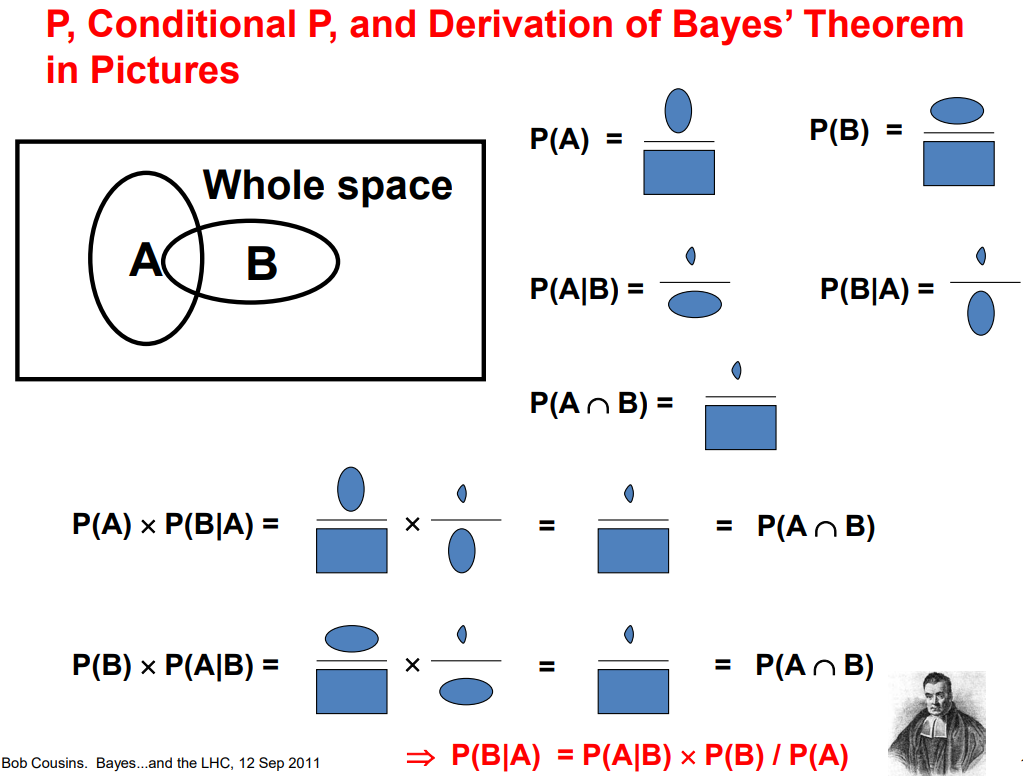
\includegraphics[width=0.9\textwidth]{bayes_rule.png}}}
		\caption{Bayes' Rule in Pictures}
		\label{bayes_rule}
	\end{figure}
	
	Let $X$ and $Y$ denote two continuous random variables. Then, the \newline \underline{conditional pdf} $p_{X|Y}(x|y)$ of $x$ given $y$ is
	
	\begin{equation*}
		p_{X|Y}(x|y) = \frac{p_{X,Y}(x,y)}{p_Y(y)}
	\end{equation*}
	
	Above important theorem can be stated in many different ways. We suppress the subscripts for convenience.
	
	\begin{equation*}
		p(x|y) = \frac{p(x,y)}{p(y)},\quad p(y|x) = \frac{p(x,y)}{p(x)}
	\end{equation*}
	
	\begin{equation*}
		\therefore p(x|y) = \frac{p(x,y)}{p(y)} = \frac{p(y|x)p(x)}{p(y)} = \frac{p(x)p(y|x)}{\int_{-\infty}^{\infty}{p(x)p(y|x)dx}}
	\end{equation*}
	
	If random variable $x$ is being determined by observing the random variable $y$, we use the notation:
	
	$p(x) = \text{"a priori" probability}$
	
	$p(y|x) = \text{conditional probability}$
	
	$p(x|y) = \text{"a posteriori" probability}$
	
	We provide a few examples of \underline{univariate} random variables below.
	
	\begin{enumerate}
		\item[(1)] \underline{Poisson:} The discrete random variable $n$ takes on integer values \newline $0,1,2,...,k,...$ till $\infty$
		
		\begin{equation*}
			\text{Pr}(n = k) = \frac{\lambda^k e^{-\lambda}}{k!},\quad\lambda > 0
		\end{equation*}
		
		$E\{n\} = \lambda$ and $\text{var}\{n\} = \lambda$
		
		\item[(2)] \underline{Binomial:} The discrete random variable $n$ takes on integer values \newline $0,1,2,...,N$.
		
		\begin{equation*}
			\text{Pr}(n = k) = \frac{N!}{k!(N-k)!}\theta^k(1 - \theta)^{(N - k)}, \quad k = 0,1,...,N
		\end{equation*}
		
		where $\theta$ is a parameter.
		
		$E\{n\} = N\theta$ and $\text{var}\{n\} = N\theta(1-\theta)$
		
		\item[(3)] \underline{Uniform:} The continuous random variable $x$ is governed by
		
		\begin{equation*}
			p(x) = \begin{cases}
				\frac{1}{(b-a)} & \text{for}\ a \leq x \leq b\\
				0 & \text{otherwise}
			\end{cases}
		\end{equation*}
		
		$E\{x\} = \left(\frac{a+b}{2}\right)$, the mid-point of the interval
		
		$var\{x\} = \frac{(b - a)^2}{12}$, one-twelfth of the square of the interval length.
		
		\item[(4)] \underline{Univariate Gaussian:} The continuous random variable $x$ has the following pdf.
		
		\begin{equation*}
			p(x) = \frac{1}{\sqrt{2\pi{\sigma_x}^2}}\text{exp}\left[-\frac{1}{2}\frac{(x-\mu_x)^2}{{\sigma_x}^2}\right]
		\end{equation*}
		
		$E\{x\} = \mu_x$ and $\text{var}\{x\} = {\sigma_x}^2$
		
		The univariate Guassian is \underline{completely} characterized by two parameters, namely, mean $\mu_x$ and variance ${\sigma_x}^2$
		
		For \underline{zero mean}, univariate Gaussian random variables, we can show the following.
		
		\begin{equation*}
			E\{x^p\} = \begin{cases}
				0 & \text{for odd}\ p\\
				\frac{p!}{\left(\frac{p}{2}\right)!2^{(p/2)}}\sigma^p & \text{for even}\ p
			\end{cases}
		\end{equation*}
			
		A univariate Gaussian pdf with mean $\mu$ and variance $\sigma^2$ is often denoted by $\mathcal{N}(\mu,\sigma^2)$
		
		The \underline{error function} $\text{erfc}(x)$ is defined as
		
		\begin{equation*}
			\text{erfc}(x) \overset{\Delta}{=} \frac{1}{\sqrt{2\pi}}\int_x^{\infty}{e^{-\frac{u^2}{2}}du}
		\end{equation*}
		
		$\text{erfc}(-\infty) = 1$, $\text{erfc}(0) = \frac{1}{2}$, $\text{erfc}(\infty) = 0$, $\text{erfc}(x) = 1 - \text{erfc}(x)$
		
		You can evaluate the error function on your calculator very accurately using the following algorithm.
		
		$\text{erfc}(x) = F(t)e^{-(x^2/2)}$
		
		$t = 1/(1 + 0.2316419x)$
		
		$F(t) = t\{0.127414796 + t\{-0.142248368 + t\{0.710706871$
		
		$+ t\{-0.726576013 + 0.530702714t\}\}\}\}$
		
		You may have to find $x$ such that
		
		$\beta = \text{erfc}(x),\quad 0 < \beta < \frac{1}{2}$
		
		Then $x$ can be obtained iteratively as below.
		
		Let $x_0$ be a guess for starting value.
		
		$t_0 = 1/(1 + 0.2316419x_0)$
		
		Find a new $x$ value from $x_0$ as
		
		\begin{equation*}
			x_1 = \left\{2\text{ln}\left[\frac{F(t_0)}{\beta}\right]\right\}^{1/2}
		\end{equation*}
		
		where $F(t)$ is the polynomial above.
		
		\item[(5)] \underline{Rayleigh:} The continuous random variable $x$ is governed by the following pdf.
		
		\begin{equation*}
			p(x) = \begin{cases}
				\frac{x}{b^2}e^{-\frac{x^2}{2b^2}} & \text{for}\ x \geq 0\\
				0 & \text{for} x < 0
			\end{cases}
		\end{equation*}
		
		\item[(6)] \underline{Gamma:} The continuous random variable $x$ is governed by the following pdf.
		
		\begin{equation*}
			p(x) = \begin{cases}
				\frac{1}{\Gamma(c)}x^{(c-1)}e^{-x} & \text{for}\ x \geq 0, c > 0\\
				0 & \text{for}\ x < 0
			\end{cases}
		\end{equation*}
		
		where the \underline{Gamma function} $\Gamma(c)$ is defined by
		
		\begin{equation*}
			\Gamma(c) \overset{\Delta}{=} \int_0^{\infty}x^{(c-1)}e^{-x}dx
		\end{equation*}
		
		Fortunately, we can use the recursion that
		
		$\Gamma(c+1) = c\Gamma(c)$ along with $\Gamma(1) = 1$, $\Gamma(\frac{1}{2}) = \sqrt{\pi}$, and $\Gamma(n) = (n-1)!$
		
		\item[(7)] \underline{Chi-squared:} The continuous random variable $x$ is governed by the following pdf.
		
		\begin{equation*}
			p(x) = \begin{cases}
				\frac{1}{2^{\beta/2}\Gamma\left(\frac{\beta}{2}\right)}x^{\left(\frac{\beta}{2} - 1\right)}e^{-\frac{x}{2}} & \text{for}\ x \geq 0\\
				0 & \text{for}\ x < 0
			\end{cases}
		\end{equation*}
		
		where $\beta$ is the \underline{number of degrees of freedom} associated with the chi-squared distribution
		
		The sum of squares of $N$ \underline{independent}, zero mean Gaussian variables with unit variance results in a chi-squared random variable with $N$ degrees of freedom
		
		Note also that if $x$ is a chi-squared random variable with $\beta$ degrees of freedom, then $(x/2)$ is a gamma random variable with the parameter \newline $c = (\beta/2)$.
		
	\end{enumerate}
		
	Two continuous random variables $x$ and $y$ are \underline{bivariate Gaussian} if their join pdf is as below.
		
	\begin{equation*}
		p(x,y) = \frac{1}{2\pi\sigma_x\sigma_y\sqrt{1-\rho^2}} \cdot
	\end{equation*}

	\begin{equation*}
		\text{exp}\left\{-\frac{1}{2(1-\rho^2)}\left[\frac{(x-\mu_x)^2}{\sigma_x^2} - \frac{2\rho(x - \mu_x)(y - \mu_y)}{\sigma_x\sigma_y} + \frac{(y - \mu_y)^2}{\sigma_y^2}\right]\right\}
	\end{equation*}
		
	$E\{x\} = \mu_x$, $E\{y\} = \mu_y$, $\text{var}\{x\} = \sigma_x^2$, $\text{var}\{y\} = \sigma_y^2$ and $\rho$ is the \newline \underline{correlation coefficient} between $x$ and $y$
		
	Note that for $\rho = 0$, we can write $p(x,y)$ as the product of $p(x)$ and $p(y)$ indicating statistical independence.
		
	For jointly Guassian random variables,
		
	$\text{uncorrelatedness} \Leftrightarrow \text{statistical independence}$
		
	$\text{Pr}\left[x\ \text{and}\ y\ \text{have the same sign}\right] = \frac{1}{2} + \frac{1}{\pi}\sin^{-1}(\rho)$
		
	For the jointly Gaussian random variables $x$ and $y$, the conditional pdf $p(x|Y=y)$ is as below.
		
	\begin{equation*}
		p(x|Y=y) = \mathcal{N}\left(\mu_x + \rho\frac{\sigma_x}{\sigma_y}(y - \mu_y), \sigma_x^2-\rho^2\sigma_x^2\right)
	\end{equation*}
		
	Note that for $\rho = 0$, $p(x|Y=y)$ is simply $\mathcal{N}(\mu_x,\sigma_x^2)$
		
	Let $x_1, x_2, ..., x_N$ be a set of \underline{independent} random variables with arbitrary distributions, means $\mu_i$ and variances $\sigma_i^2$. Then form a new random variable $y_N$ given by
		
	\begin{equation*}
		y_N = \frac{(x_1 + x_2 + \cdots + x_N) - (\mu_1 + \mu_2 + \cdots + \mu_N)}{\sqrt{\sigma_1^2 + \sigma_2^2 + \cdots + \sigma_N^2}}
	\end{equation*}
		
	Then, under general conditions, the CDF of $y_N$ approaches the CDF of a unit Gaussian as $N$ goes to infinity (\underline{Central Limit Theorem}).
		
	The random variables $x_1,x_2,...,x_M$ are said to be \underline{jointly Gaussian} if their join pdf is given by
		
	\begin{equation*}
		p(\mathbf{x}) = \frac{1}{\sqrt{(2\pi)^M|\mathbf{\Sigma_x}|}}\text{exp}\left\{-\frac{1}{2}(\mathbf{x} - \mathbf{\boldsymbol{\mu}_x})^T\mathbf{\Sigma_x}^{-1}(\mathbf{x} - \mathbf{\boldsymbol{\mu}_x})\right\}
	\end{equation*}
		
	Here $E\{\mathbf{x}\} = \mathbf{\boldsymbol{\mu}_x}$ and $\text{cov}(\mathbf{x}) = \mathbf{\Sigma_x}$, $\mathbf{x} = \begin{bmatrix}x_1,x_2,...,x_M\end{bmatrix}^T$
		
	$|\cdot|$ denotes the determinant of the matrix.
		
	This M-variate Gaussian pdf is also denoted by $\mathcal{N}_M(\mathbf{\boldsymbol{\mu}_x},\mathbf{\Sigma_x})$ where the subscript denotes the number of random variables.
		
	If $\mathbf{Y} = \mathbf{Ax}$, then we can show that $\mathbf{Y}$ is also \underline{multivariate Gaussian} with
		
	$E\{\mathbf{Y}\} = \mathbf{A\boldsymbol{\mu}_x}$ and $\mathbf{\Sigma_y} = \mathbf{A\Sigma_x}\mathbf{A}^T$
		
	The multivariate Guassian is a very popular model because of the following features.
		
	\begin{enumerate}
	
		\item[(i)] Central limit theorem
		
		\item[(ii)] Linear transforms preserve the Gaussian nature
		
		\item[(iii)] Parameterized completely by $\boldsymbol{\mu}$ and $\mathbf{\Sigma}$.
		
		\item[(iv)] Conditional pdfs of components are also Gaussian. 
		
	\end{enumerate}
	
	A \underline{complex Gaussian random variable} $z$ is actually made up of two random variables $x$ and $y$ as below.
	
	$z = x + jy$
	
	$E\{x\} = 0$, $E\{y\} = 0$, $\text{var}\{x\} = (\sigma^2/2)$, $\text{var}\{y\} = (\sigma_y^2/2)$, $\text{cov}(X,Y) = 0$.
	
	Of course, $X$ and $Y$ are Gaussian.
	
	Then, note that $E\{z\} = 0$, $E\{zz\} = 0$, $E\{z^*z^*\} = 0$ and $E\{zz^*\} = \sigma^2$, where $*$ denotes the complex conjugate.
	
	The characteristic function of $\mathcal{N}_M(\boldsymbol{\mu}, \mathbf{\Sigma})$ is
	
	$\Phi_\mathbf{x}(\mathbf{u}) = \text{exp}[j\boldsymbol{\mu}^T\boldsymbol{\mu} - \frac{1}{2}\boldsymbol{\mu}^T\mathbf{\Sigma}^{-1}\boldsymbol{\mu}]$
	
	Let $\mathbf{X} = \begin{bmatrix}\mathbf{X_1} \\ \mathbf{X_2} \end{bmatrix}$ be distributed as $\mathcal{N}_M(\boldsymbol{\mu},\mathbf{\Sigma})$ with $\boldsymbol{\mu} = \begin{bmatrix} \mathbf{\boldsymbol{\mu}_1} \\ \mathbf{\boldsymbol{\mu}_2} \end{bmatrix}$ and $\mathbf{\Sigma} = \begin{bmatrix} \mathbf{\Sigma_{11}} & \mathbf{\Sigma_{12}} \\ \mathbf{\Sigma_{21}} & \mathbf{\Sigma_{22}} \end{bmatrix}$ and $|\mathbf{\Sigma_22}| > 0$. Then the conditional distribution of $\mathbf{X_1}$, given $\mathbf{X_2} = \mathbf{x_2}$ is also \underline{Gaussian} with mean vector $\mathbf{\boldsymbol{\mu}_1} + \mathbf{\Sigma_{12}}\mathbf{\Sigma_{22}}^{-1}(\mathbf{x_2} - \mathbf{\boldsymbol{\mu}_2})$ and covariance matrix $\mathbf{\Sigma_{11}} - \mathbf{\Sigma_{12}}\mathbf{\Sigma_{22}}^{-1}\mathbf{\Sigma_{21}}$. Note that the covariance matrix does not depend on the conditioning value $\mathbf{x_2}$.
	
	If the random vector $\mathbf{X}$ is distributed according to $\mathcal{N}_M(\boldsymbol{\mu},\mathbf{\Sigma})$ with $|\mathbf{\Sigma}| > 0$, then:
	
	\begin{enumerate}
		\item[(i)] $(\mathbf{X} - \boldsymbol{\mu})^T\mathbf{\Sigma}^{-1}(\mathbf{X} - \boldsymbol{\mu})$ is distributed according to a \underline{chi-squared} distribution with $M$ degrees of freedom.
		
		\item[(ii)] The $\mathcal{N}_M(\boldsymbol{\mu}, \mathbf{\Sigma})$ assigns probability $(1 - \alpha)$ to the solid ellipsoid \newline $\{\mathbf{X}: (\mathbf{X} - \boldsymbol{\mu})^T\mathbf{\Sigma}^{-1}(\mathbf{X} - \boldsymbol{\mu}) \leq \chi_M^2(\alpha)\}$, where $\chi_M^2(\alpha)$ denotes the upper ($100\alpha$)th percentile of the $\alpha^2$ distributions (chi-squared with $M$ d.o.f.).
		
	\end{enumerate}
	
	\underline{Whitening Transform:} Let $\mathbf{x}$ be a M-variate Gaussian with mean $\mathbf{\boldsymbol{\mu}_x}$ and covariance $\mathbf{\Sigma_x}$.
		
	Let $\mathbf{\Sigma_x}\mathbf{\Phi_j} = \lambda_j\mathbf{\Phi_j}$, $j = 1,2,...,M$.
	
	$\mathbf{\Phi_i}^T\mathbf{\Phi_i} = \delta_{ij}$, $1 \leq i,j \leq M$ where
	
	\begin{equation*}
		\delta_{ij} = \begin{cases}
			1 & \text{for}\ i = j \\
			0 & \text{for}\ i \neq j
		\end{cases}
	\end{equation*}
	
	Let $\mathbf{A}$ be a $M \times M$ matrix with the eigenvector $\mathbf{\Phi_i}$ as its ith row.
	
	\begin{equation*}
		A = \begin{bmatrix}\mathbf{\Phi_1}, \mathbf{\Phi_2},...,\mathbf{\Phi_M}\end{bmatrix}^T
	\end{equation*}
	
	Let $\mathbf{Y} = \mathbf{Ax}$. Then $\mathbf{\Sigma_y} = \mathbf{A\Sigma_x}\mathbf{A}^T = \text{Diag}(\lambda_1,\lambda_2,...,\lambda_M)$.
	
	Since $\mathbf{\Sigma_y}$ is diagonal, all elements of $\mathbf{Y}$ are \underline{uncorrelated}. Because of the Gaussian pdf, this also implies \underline{statistical independence}.
	
	By multiplying the components of $\mathbf{Y}$ by proper scalars, the covariance matrix can be made into an identity matrix. The resulting random variables are statistically independent Gaussian variables of unit variance.
	
	This procedure known as the "whitening transform" facilitates the analysis when dealing with multivariate Gaussian distributions.
\end{document}